\documentclass[a4paper,10pt,twoside, openright]{book}
\usepackage[english]{babel}
%\usepackage[utf8]{inputenc}
\usepackage{indentfirst}
\usepackage{graphicx}
\usepackage{epigraph}
\usepackage{atlasphysics}

\usepackage{lineno}
%\linespread{1.2}                        %comando per impostare l'interlinea


%\usepackage{ulem} %sostituisce l'effetto sottolineatura all'effetto corsivo nel comando \emph{} e risolve il problema delle righe che non si spezzano

\usepackage{multirow}
\usepackage{enumerate}

\usepackage[hdivide={3cm, *, 3cm}, vscale=0.65, bindingoffset=1cm]{geometry}
\usepackage{chngpage}

\usepackage[format=hang,indention=-2cm,labelfont=bf]{caption}%per delle caption più carine
\usepackage{booktabs}
\usepackage{longtable}
%\usepackage{pdflscape} 
%\usepackage[pdftex]{lscape}
\usepackage{lscape}
\usepackage{slashed}

\usepackage{listings}
\lstset{language=C}

\hyphenation{ca-lo-ri-me-ter ca-lo-ri-me-ters}%serve per la sillabazione: tra parentesi 

\setlength{\headheight}{15pt}
\usepackage{pict2e}
%\usepackage{guit}

%\usepackage{natbib}
%\bibliographystyle{unsrt}
%\usepackage[babel]{csquotes}
%\usepackage[style=numeric,sorting=none]{biblatex}
%\bibliography{biblio}


%MATHS
\usepackage{amssymb}
\usepackage{amsmath}
\usepackage{latexsym}
\usepackage{amsthm}
 \newcommand{\sgn}{\mathop{\mathrm{sgn}}}
\usepackage{slashed}
\usepackage[usenames,dvipsnames,svgnames,table]{xcolor}

%\usepackage[T1]{fontenc}
%\usepackage{microtype}

\usepackage{fancyhdr}
\pagestyle{fancy}

\usepackage{eso-pic}

\usepackage{url}
\usepackage[ps2pdf,bookmarks=true,bookmarksnumbered=false,% true means bookmarks in left window are numbered
bookmarksopen=false, % true means only level 1 are displayed.
colorlinks=true,linkcolor=webred]{hyperref}
%\usepackage[pdfborder={0 0 0 0}]{hyperref}
\definecolor{webgreen}{rgb}{0, 0.5, 0} % less intense green
\definecolor{webblue}{rgb}{0, 0, 0.5} % less intense blue
\definecolor{webred}{rgb}{0.5, 0, 0} % less intense red

%END OF PACKAGES

%per includere il frontespizio (ottenuto in pdf a parte)
\newcommand\BackgroundPic{
\put(0,0){
\parbox[b][\paperheight]{\paperwidth}{%
\vfill
\centering

\includegraphics[width=\paperwidth,height=\paperheight,
keepaspectratio]{smallstuff/frontespizio}%
\vfill
}}}

\def\bra#1{\mathinner{\langle{#1}|}}
\def\ket#1{\mathinner{|{#1}\rangle}}
\def\braket#1{\mathinner{\langle{#1}\rangle}}
\def\Bra#1{\left<#1\right|}
\def\Ket#1{\left|#1\right>} 
\newcommand{\Overline}[2][1]{%
  {}\mkern#1mu \overline{\mkern-#1mu #2 \mkern-#1mu}\mkern#1mu {}} 
\DeclareMathAlphabet{\mathpzc}{OT1}{pzc}{m}{it}

%per avere l'indice senza numeri di pagina
\makeatletter 
 \newcommand{\cleantableofcontents}{% 
   \clearpage\begingroup 
   \let\ps@plain\ps@empty\pagestyle{empty}% 
   \tableofcontents\clearpage\endgroup} 
 \makeatother

%per lo stile dei capitoli
\makeatletter
\def\thickhrulefill{\leavevmode \leaders \hrule height 1ex \hfill \kern \z@}
\def\@makechapterhead#1{%
  \vspace*{10\p@}%
  {\parindent \z@ 
    {\raggedleft \reset@font
      \scshape \@chapapp{} \thechapter\par\nobreak}%
    \par\nobreak
    \vspace*{30\p@}
    \interlinepenalty\@M
    {\raggedright \Huge \bfseries #1}%
    \par\nobreak
    \hrulefill
    \par\nobreak
    \vskip 100\p@
  }}
\def\@makeschapterhead#1{%
  \vspace*{10\p@}%
  {\parindent \z@ 
    {\raggedleft \reset@font
      \scshape \vphantom{\@chapapp{} \thechapter}\par\nobreak}%
    \par\nobreak
    \vspace*{30\p@}
    \interlinepenalty\@M
    {\raggedright \Huge \bfseries #1}%
    \par\nobreak
    \hrulefill
    \par\nobreak
    \vskip 100\p@
  }}

\renewcommand{\chaptermark}[1]{\markboth{\thechapter. \ #1}{}}
\renewcommand{\sectionmark}[1]{\markright{\thesection.\ #1}}
\fancyhf{}
\fancyhead[LO]{\small \nouppercase{\rightmark}}
\fancyhead[RE]{\small \nouppercase{\leftmark}}
\fancyhead[RO , LE]{ \thepage}



\begin{document}
\linenumbers

\frontmatter
% Inizio Numerazione Romana
%\pagenumbering{roman}

\begin{titlepage}
\begin{adjustwidth}{-4cm}{-3cm}
\AddToShipoutPicture*{\BackgroundPic}
\end{adjustwidth}
\end{titlepage}

\clearpage{\pagestyle{empty}\cleardoublepage}

\thispagestyle{empty}

\null\vspace{\stretch{1}}
\begin{flushright}
\textit{A tempi migliori}
\vspace{\stretch{1}}\null

\begin{minipage}{.8\textwidth}\footnotesize
\begin{description}
\item[Professore:]  Lei ha una qualche ambizione?
\item[Nicola:] Ma\dots Non\dots
\item[Professore:] E Allora vada via\dots Se ne vada dall'Italia. Lasci l'Italia finch\'e \`e in tempo. Cosa vuole fare, il chirurgo?
\item[Nicola:] Non lo so, non ho ancora deciso\dots
\item[Professore:] Qualsiasi cosa decida, vada a studiare a Londra, a Parigi\dots Vada in America, se ha le possibilit\`a, ma lasci questo Paese. L'Italia \`e un Paese da distruggere: un posto bello e inutile, destinato a morire.
\item[Nicola:] Cio\`e, secondo lei tra poco ci sar\`a un'apocalisse?
\item[Professore:] E magari ci fosse, almeno saremmo tutti costretti a ricostruire\dots Invece qui rimane tutto immobile, uguale, in mano ai dinosauri. Dia retta, vada via\dots
\end{description}

\begin{flushright}
\textit{da} La meglio Giovent\`u \textit{di M.T. Giordana (2003)}
\end{flushright}
%\`o \`o - à \`a - è \`e - ì \`i - ù \`u - é \'e


\end{minipage}
\end{flushright}


\clearpage{\pagestyle{empty}\cleardoublepage}

\clearpage{\pagestyle{empty}\cleardoublepage}

\chapter*{Introduccion}\label{chap:introES}



\clearpage{\pagestyle{empty}\cleardoublepage}

% Indice

\pdfbookmark[1]{Index}{Index}
\cleantableofcontents

% Elenco delle Figure
%\addcontentsline{toc}{section}{\listfigurename}
%\listoffigures

\clearpage{\pagestyle{empty}\cleardoublepage}

\phantomsection
\addcontentsline{toc}{chapter}{Introduction}
\clearpage{\pagestyle{empty}\cleardoublepage}

\chapter*{Introduction}\label{chap:intro}

%\vskip-2.5cm

%\subsection*{Part I}
July 4th, 2012, represents a milestone for high-energy physics,
being the date when the ATLAS and CMS experiments at CERN announced
the discovery of a new particle consistent with a Standard Model Higgs
boson with mass $m_H\sim 125\gev$. Is it going to be celebrated, 20 years
from now, as the beginning of a new era of discoveries or as the 
end of the adventure? Is there something {\it more}, out there, in 
the outer space or 100~m underground, awaiting for being discovered?
As outlined in Chapter~\ref{chap:TH} there is quite some evidence
something must be there lying ``beyond the Standard Model''. 
A successful theory finally completed
by the identification of the Higgs boson, 
the Standard Model as it is still leaves too many questions
unanswered. What is ``Dark Matter'', this exotic form of energy density different
from atoms, being immune to electromagnetic interactions, but which
is known to account for $\sim$27\% of the total matter in the Universe?
After the Big Bang, what caused the asymmetry in the production of particles vs
antiparticles that made matter prevail over antimatter?
Why is the top quark so much heavier than the other quarks? Why is the
Higgs boson so much lighter than the Planck mass?

It was to find an explanation to this puzzle that the 
Large Hadron Collider project was initiated 20 years ago. The ATLAS
collaboration then started the design of the detector described in
Chapter~\ref{chap:atlas}, outlining an ambitious physics program
in which the search for the Higgs boson was ``just'' the first bullet
of the list.
The LHC first run was on the 20th of November 2009, with the ATLAS
experiment beginning to record data from these early proton-proton
collisions at a \cme\ of $900$~GeV just three days later.
Since then, outstanding performances of both the accelerator
and the detector allowed to collect a huge amount of data
from proton-proton collisions at increasing center of mass energies, reaching in
2012 a total of $\sim$20~\ifb\ at a \cme\ of 8~TeV.

%During the long time that passed between the detector construction
%and when the real data became available in 2009, analyses relied on
%data collected during test-beam runs and on Monte Carlo simulation.
However, this large amount of data alone would 
not tell much if it were not possible to
compare them to precise theoretical predictions.
Chapter~\ref{chap:mc} describes the Monte Carlo techniques used
to obtain simulated samples of either ``Standard Model'' %processes 
or ``new physics'' events. 
%Monte Carlos are powerful tools that used with the purpose of 
%calibrating the detector, 
%modeling the contributions to some particular channel
%allow 
Starting from the computation of the matrix element of a 
particular process, Monte Carlo tools
are combined to obtain the complete picture of how the
event of interest develops, including as a last step
the simulation of the particles interactions with the
detector material.

Whether real data or Monte Carlo simulated samples, at
the ``raw'' level events are simple digital outputs, coming respectively
from the real or simulated response of the read-out electronics
of the different ATLAS detector subsystems. How these outputs
are assembled into physical objects is described in Chapter~\ref{chap:objects},
where the reconstruction process is explained.
The outcome is a dataset containing all the information needed
about physics objects such as leptons, jets and energy 
imbalance of the event,
ready to be processed by analyses.


%\subsection*{Part II}
%The object of this dissertation is then introduced in Chapter~\ref{chap:vlq}.
Using these kind of datasets, 
%motivated by more than one theoretical proposals for beyond Standard Model physics, 
the Exotics group of the ATLAS collaboration defined a search strategy 
for exotic heavy quarks different from the first three generations 
%in that they do not show a chiral behavior under the electroweak group transformations.
%These quarks are 
and called ``vector-like''. Even though these quarks are
predicted in various proposed extentions of the Standard Model, 
like extra-dimensions or composite Higgs
models, no details on their masses are given and their decay branching fractions
are very model dependent. Searches aiming at inclusivity 
must therefore rely as little as possible on 
assumptions from the model, and this is the approach chosen for the
two searches in the single lepton channel
for pair-produced heavy vector-like top partners 
presented in this dissertation. The general quasi-model independent
strategy common to the two analyses, performed analyzing 
$\sim$14~\ifb\ of data from proton-proton collisions at the
 \cme\ $\rts=8\tev$ recorded during the year 2012 
at the ATLAS experiment, is presented in
Chapter~\ref{chap:vlq}.

The search for pair-produced heavy vector-like top partners
where at least one of them decays into a $W$ boson and a bottom
quark is detailed in Chapter~\ref{chap:wbx}. The key point in
this analysis is the reconstruction of the $W$ boson from its
hadronic decay products which allows for the reconstruction
of the heavy quark mass, a very good discriminating variable between
signal and Standard Model background processes.

Chapter~\ref{chap:htx} presents the search for 
pair-produced heavy vector-like top partners
where at least one of them decays into a Standard Model Higgs
boson and a top quark. In this case the main decay of the Higgs
boson into two bottom quarks is exploited resulting in a
final state signature characterized by a high number of recontructed
jets, where a large fraction of them is identified as originating
from the hadronization of bottom quarks.

While the individual results from the searches
are presented in the respective chapters, higher
sensitivity is achieved combining the two analyses.
This is described in Chapter~\ref{chap:results},
and the result of these searches is compared with
other similar searches exploiting multi-lepton signatures.
%where also a prospect is given of a potential combination of these searches with the other analyses performed by ATLAS searching for heavy vector-like quarks in final states with two leptons.






%\newpage
%\phantomsection
%\addcontentsline{toc}{section}{Acknowledgement}
\subsubsection*{Personal contributions and acknowledgement}

The results presented in this dissertation represent
a small sample of the achievements made possible by
the combined effort of many, many people. The ATLAS
collaboration itself consists of $\sim$3000 scientists,
working in different subgroups. In particular,
the author of this dissertation participated to calibration
and performance studies of the hadronic calorimeter
and to the improvement of data-driven estimation of
multi-jet backgrounds for analyses with top quarks 
decaying in the single-muon channel. Regarding
the two analyses object of this dissertation, the author
has been amongst the main analyzers, implementing and
running the signal selection and statistical analysis and
performing the needed cross checks for the good modeling
of background predictions. % and for Monte Carlo signal modeling.
The results are documented in two preliminary 
notes~\cite{ATLAS-CONF-2013-060,ATLAS-CONF-2013-018}.
The work for the final analyses to be published is still on-going at
the time of the writing of this dissertation.
The author also significantly participated to a previous,
published analysis~\cite{ATLAS:2012qe}
performed on the data from lower \cme\ 
proton-proton collisions which pioneered searches for
heavy vector-like quarks in ATLAS.

A particular acknowledgement goes to the ``IFAE-top''
group, present and former members, for their fundamental
contributions to the common analysis framework used
for these searches.


\clearpage{\pagestyle{empty}\cleardoublepage}


\mainmatter

\clearpage{\pagestyle{empty}\cleardoublepage}

\chapter{The ATLAS experiment at the Large Hadron Collider}\label{chap:atlas}

The analyses presented in this dissertation have been performed analyzing data from 
proton-proton (p-p) collisions at the \cme $\rts=8\tev$ recorded during the year 2012 
at the ATLAS experiment~\cite{Aad:2008zzm}. In the following Chapter we will briefly 
describe the main features of the detector, located at the CERN laboratories in Geneva,
Switzerland.

The experimental facilities are situated at Point~1 along the Large Hadron Collider 
(LHC)~\cite{lhc} 27~km long ring, shown in Figure~\ref{fig:lhcring}. The accelerator
tunnel can reach an underground depth of 175~meters and is spread between Swiss
and French territory, while the cave where ATLAS is allocated is about 100~meters 
underground in the CERN Swiss site of Meyrin. 

\begin{figure}[tb]\begin{center}
	\subfigure{\label{fig:lhcring}
  	\includegraphics[width=0.8\textwidth]{detector/figures/ring.eps}}
	\caption{A schematic showing the accelerator complex at CERN. Protons are
        extracted from Hydrogen gas and injected in the first machine, the linear 
        accelerator LINAC2 that starts the acceleration chain. When protons reach
        an energy of 50\mev they are injected into the Proton Synchrotron Booster
        (PSB) and accelerated up to the energy of 1.4\gev. The second circular
        accelerator, the Proton Synchrotron (PS) brings the energy of the protons
        to 25\gev previous to injecting them into the last machine before the LHC,
        the Super Proton Synchrotron (SPS). Protons of 450\gev finally enter the
        LHC where they are boosted to energies of up to 4\tev.
        The four main LHC experiments are shown on the collider ring.}
\end{center}\end{figure}

The LHC program was approved by CERN Council in 1994, followed by the approval of
the four main experiments physics programs: ATLAS~\cite{Aad:2008zzm} and CMS~\cite{cms}
in 1996; ALICE~\cite{alice} in 1997; LHCb~\cite{lhcb} in 1998.
Works towards the installation of the most powerful particle accelerator of the world
started when the Large Electron Positron Collider (LEP) was dismantled in 2000 to 
give up its place in the tunnel to the LHC, which was then fully operational by 2008.

The LHC is composed of eight arcs 2.7~km long, each of which contains 154 dipole 
magnets, whose function is to  bend the beams along the circular trajectory, and
49 quadrupole magnets, that focus the beam. These superconducting magnets operate
at a temperature of 1.9~K, maintained by means of liquid Helium vessels.
Eight insertions are placed inbetween the arches. Each insertion has a specific
role that characterizes its design and can be injection, beam dumping, beam cleaning,
or ``physics'', i.e. make the beams collide within an experiment.

First proton beams were circulated on 10th September 2008 and right on the verge of
getting the first collisions at a \cme $\rts=900\gev$ nine days later, an electrical
connection joining superconducting wires of a dipole and a quadrupole
failed. This caused the release of liquid Helium in the insulating vacuum,
resulting in an explosion that severely damaged the machine.
After more than one year devoted to repair the damage and consolidate the security,
on 30th November 2009 the LHC became the world's highest energy particle 
accelerator\footnote{\url{http://press.web.cern.ch/press/PressReleases/Releases2009/PR18.09E.html}}:
\begin{quotation}\small
Geneva, 30 November 2009. CERN's Large Hadron Collider has today become the world’s highest energy particle accelerator, having accelerated its twin beams of protons to an energy of 1.18 TeV in the early hours of the morning. This exceeds the previous world record of 0.98 TeV, which had been held by the US Fermi National Accelerator Laboratory’s Tevatron collider since 2001. It marks another important milestone on the road to first physics at the LHC in 2010.
\end{quotation}





The main performance figure of merit for an accelerator is the luminosity, the 
instantaneous luminosity $\mathcal L$ being defined as 
\begin{equation}\label{eq:lumiN}
\mathcal{L}\times\sigma=\dfrac{dN}{dt}=f\times n\dfrac{N_1\times N_2}{A}\times\sigma.
\end{equation} 
Here $dN/dt $ is the event rate of a certain process and $\sigma$ is its cross 
section. This rate is directly proportional to the the frequency $f$, the number 
of bunches $n$ and the number of particles in the two bunches $N_1, N_2$, and
inversely proportional to the beam cross-section $A$.

Integrating over the accelerator active time (a ``fill'', when stable beams are kept
colliding) gives the \textit{integrated luminosity}, relating the total number 
of produced events $N_{tot}$ to the cross-section:
\begin{equation}\label{eq:intLumi}
\int \mathcal L dt  = \dfrac{N_{tot}}{\sigma} 
\end{equation}


\clearpage{\pagestyle{empty}\cleardoublepage}


\section{Going beyond the SM with vector-like quarks}\label{sec:THvlq}

\cite{AguilarSaavedra:2009es,Martin:2009bg}

\subsection{Production}\label{sec:vlqprod}


\subsection{Decay}\label{sec:vlqdecay}





\clearpage{\pagestyle{empty}\cleardoublepage}
%\clearpage{\pagestyle{empty}\cleardoublepage}

%\chapter{Object reconstruction}\label{chap:objects}
\section{Object reconstruction}\label{chap:objects}

After having described the ATLAS detector, in the following Section we will
explain how object (electrons, muons, jets and the missing transverse energy \met) 
are reconstructed to be used in physics analyses. In addition details from
selections common to the analyses presented in this dissertation are given.


%\section{Electrons}\label{sec:electrons}
\subsection{Electrons}\label{sec:electrons}
Electrons are reconstructed for pseudorapidities up to $|\eta| = 2.5$, where
information from the ID is available, matching a track with an energy deposit
(cluster) in the electromagnetic calorimeter. 

To identify tracks from ID points an inside-out algorithm is used, starting from a 
seed of three aligned hits in the pixel detector or in the SCT. Five fundamental parameters,
shown and described in Figure~\ref{fig:trackpar}, are computed and used for the subsequent 
steps of hits association. The candidate track must be 

\begin{figure}[tb]\begin{center}
	\subfigure[]{
  	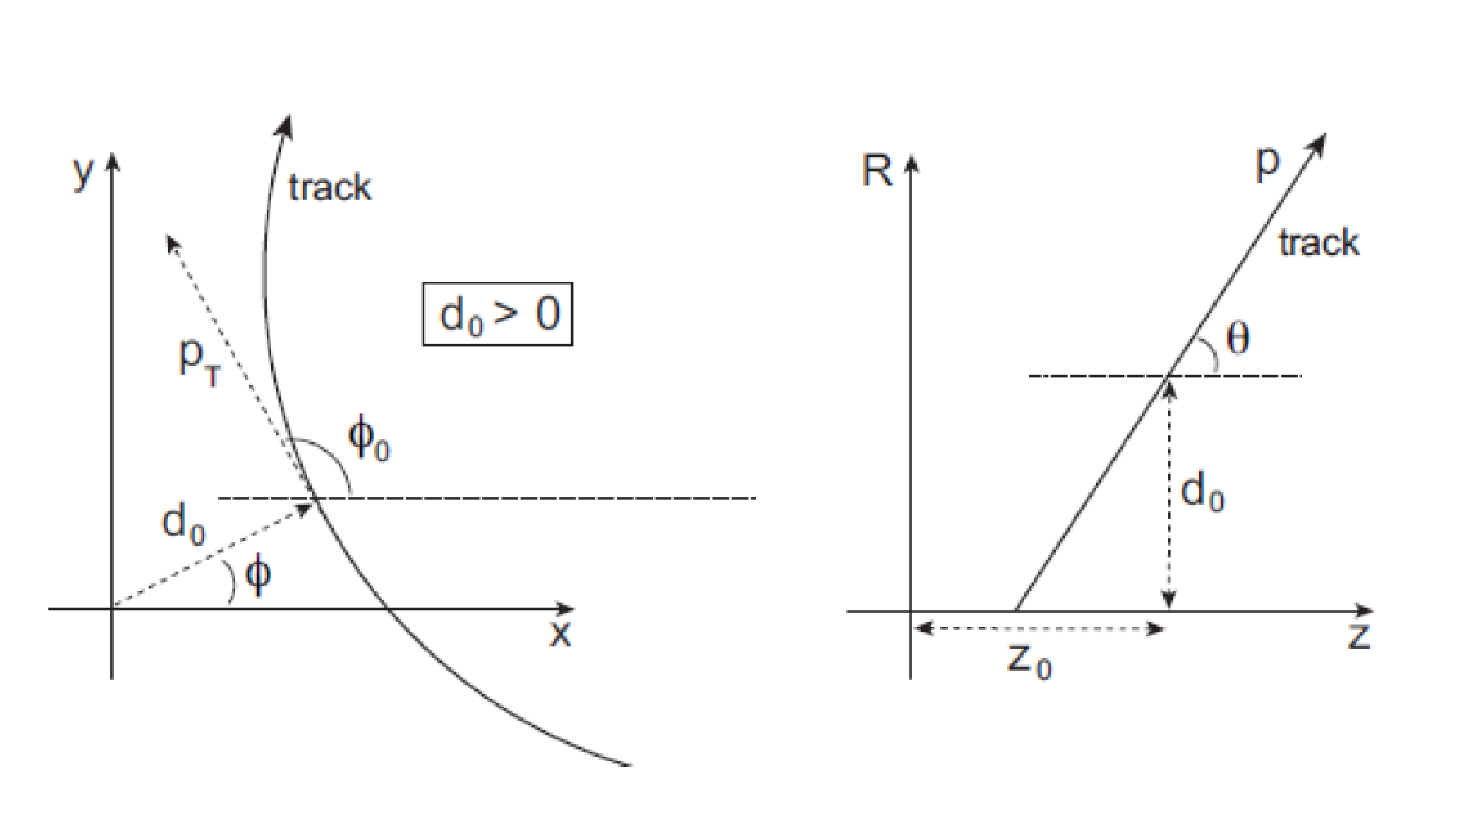
\includegraphics[width=0.7\textwidth]{objectsreconstruction/figures/tracks}}
	\caption{Schematic drawings of the parameters used for track reconstruction in the XY and $R$Z planes (left and right respectively).
          The parameters are: $q/p$, the charge divided by the momentum; $\theta$, or more used $\eta$, the angle
          with respect to the Z axis in the $R$Z plane measured from the perigee; $\phi_0$, the angle 
          with respect to the X axis in the XY plane measured from the perigee; $d_0$, the impact parameter, 
          or perigee with respect to the Z axis in the XY plane; $z_0$, Z component of the perigee.\label{fig:trackpar}}
\end{center}\end{figure}


Clusters are built starting from
$\Delta\eta\times\Delta\phi=0.025\times0.025$ single energy deposits summing
up into towers. Adjacent towers form clusters of $3\times7$ cells units in $\eta\times\phi$
in $|\eta|<1.4$ and $5\times5$ further.




excluding the transition region $1.37<|\eta| <1.52$
with inactive material.



%\section{Muons}\label{sec:muons}
\subsection{Muons}\label{sec:muons}



%\section{Jets}\label{sec:jets}
\subsection{Jets}\label{sec:jets}


%\section{Missing Transverse Energy}\label{sec:met}
\subsection{Missing Transverse Energy}\label{sec:met}


\clearpage{\pagestyle{empty}\cleardoublepage}
\clearpage{\pagestyle{empty}\cleardoublepage}

\chapter{Monte Carlo simulation}\label{chap:mc}


\section{Parton shower}\label{sec:partonshower}

\section{Hadronization}\label{sec:hadronization}

\section{Underlying-event}\label{sec:underlyingevent}

\section{Generators}\label{sec:generators}



\clearpage{\pagestyle{empty}\cleardoublepage}
\clearpage{\pagestyle{empty}\cleardoublepage}

\chapter{Preliminary search for \TTbar\ pairs decaying to $Wb+X$}\label{chap:wbx}

\section{Boosted $W$ reconstruction}\label{sec:boostedW}

\section{Control regions}\label{sec:wbxCR}

\section{Event selection}\label{sec:wbxEVT}

%\section{}\label{sec:}

%\section{}\label{sec:}

\section{Systematics}\label{sec:wbxSYS}


\clearpage{\pagestyle{empty}\cleardoublepage}
\clearpage{\pagestyle{empty}\cleardoublepage}

\chapter{$T\bar{T}\to Ht+X$}\label{chap:htx}


\clearpage{\pagestyle{empty}\cleardoublepage}
\clearpage{\pagestyle{empty}\cleardoublepage}

\chapter{Statistical treatment and Results}\label{chap:results}



\section{The CL$_s$ method}\label{sec:cls}


%\section{Systematics}\label{sec:systematics}


\section{Results}\label{sec:results}


\clearpage{\pagestyle{empty}\cleardoublepage}

\phantomsection
\addcontentsline{toc}{chapter}{Conclusions}
\clearpage{\pagestyle{empty}\cleardoublepage}

\chapter*{Conclusions and outlook}\label{chap:conclusions}

\vskip-1.5cm

Two quasi-model independent searches for 
pair production of vector-like top partners 
in proton-proton collisions at a \cme\ of 8~\tev\ 
have been presented in this dissertation. The final states considered
for both analyses involve one lepton and many jets but different
strategies are adopted in order to achieve sensitivities in different
corners of the decay phase space. Indeed, a peculiar fact for these
searches that has been stressed many times over these pages is the 
unpredicted nature of the heavy vector-like top partners model. 
As a direct consequence, the two analyses have been designed
and developed to be optimized for a particular decay mode and
to have orthogonal channels in order to allow
for a combined search that could exploit the specific sensitivities.

Three particular models, interesting from a theoretical point
of view (but not for this more favoured than others), are considered
over the two analyses: the chiral fourth-generation, with 
BR$(T\to Wb)=1$ for any value of the heavy quark mass; 
the singlet vector-like, with BR$(T\to Wb)\sim 0.5$ and 
BR$(T\to Ht)\sim 0.3$ for almost all
values of the heavy quark mass considered in the searches;
the doublet vector-like, with BR$(T\to Wb)= 0$ and 
BR$(T\to Ht)\in$ [0.50, 0.75] for all the values of the heavy quark mass.
In the \wbx\ analysis, it was possible to exclude at a 95\% CL
pair-produced chiral fourth-generation top partners and vector-like
$Y$ quarks with masses up to 740~\gev, and pair-produced vector-like 
singlet top partners with  masses up to 505~\gev.
In the \htx\ analysis, it was possible to exclude at a 95\% CL
pair-produced vector-like singlet and doublet top partners with 
masses up to 640~\gev\ and 790~\gev\ respectively.
When the two analyses are combined, the observed exclusion limit
for the only model where both analyses are sensitive, the
vector-like singlet $T$, is pushed $\sim$30~\gev\ further the
best result of the two, obtained by the \htx\ analysis,
achieving a 95\% CL exclusion of pair-produced vector-like singlet 
top partners with masses up to 670~\gev. While this might not
look like a significant improvement, the power of the combination
of the two searches is evident looking at the coverage of the
two-dimensional branching ratio plane, where  95\% CL exclusion is set for
pair-produced vector-like top partners with masses up to 550~\gev\ 
independently from the model, and also the plane for the 600~\gev\ mass
point is almost fully excluded. This strongly encourages to perform,
in the future, full combination of searches for vector-like quarks.

The mass range excluded at 95\% CL up to now
is getting closer and closer to the point where pair-production
of vector-like quarks will start to be disfavoured with respect
to single production. In this sense, while it is desirable to continue to
exploit the experience achieved up to now with the searches for
pair-produced vector-like quarks in the single lepton and multi-lepton
channels, it is a good idea to start designing searches for
single-produced vector-like quarks for LHC Phase-II.
Further improvements are possible for the searches
presented in this dissertation without changing the core of
the analysis strategies. During Phase-II they will benefit
of the increased \cme\ available for heavy quark production
in pp collisions with \rts=14~\tev\ and of the high integrated
luminosity (100~\ifb\ of data are expected over three years
of operation). With high luminosity comes the challenge of
dealing with higher pile-up, but considering that vector-like
quark searches involve high-\pt\ objects this should not
represent a major issue.

Besides the great discovery potential, the combination
of multiple searches will provide useful insights on the
exotic quark properties, like their quantum numbers or
the measurement of their branching ratios. 
Adding searches for single production of vector-like quarks
would also allow to measure the electroweak couplings of
these particles with the Standard Model quarks from the third generation.
Finally, these searches are even more interesting since
they will probe a wide range of
signatures that are often shared with other new physics
scenarios. Given the fact that during these last successful years
of LHC operation no hints on what lies ``beyond the Standard Model''
have emerged, the winning strategy is for sure not to confine ourselves 
to exclusive models.


\clearpage{\pagestyle{empty}\cleardoublepage}

\appendix

\clearpage{\pagestyle{empty}\cleardoublepage}

\chapter{}\label{appA:}


\clearpage{\pagestyle{empty}\cleardoublepage}

\clearpage{\pagestyle{empty}\cleardoublepage}

\chapter{}\label{appB:}


\clearpage{\pagestyle{empty}\cleardoublepage}

%\phantomsection
%\addcontentsline{toc}{chapter}{Ringraziamenti}
%\input{smallstuff/ringraziamenti}

\clearpage{\pagestyle{empty}\cleardoublepage}


\backmatter

%\nocite{}
\phantomsection
\addcontentsline{toc}{chapter}{Bibliography}

\bibliographystyle{woc}
\bibliography{bibliografy/biblio}

\clearpage{\pagestyle{empty}\cleardoublepage}



\end{document}
